%! TEX root = main.tex

\graphicspath{{00_Images/06_chapter/}}

\chapter{Sound Radiation}
\label{ch:sound_radiation}

The previous chapter established how mean acoustic power depends on the real part of the acoustic radiation impedance. This chapter examines what that impedance actually looks like for the two fundamental idealized sources: the plane wave (an infinite, spatially uniform radiator) and the pulsating sphere (a compact omnidirectional source). It then applies the more realistic model of a rigid circular piston mounted in an infinite baffle, which closely approximates the behavior of a loudspeaker cone. The chapter concludes by showing that the air in front of the piston contributes a real, frequency-dependent mass load to the mechanical system, lowering the resonance frequency from the value that would be obtained in vacuum.

\section{Specific Acoustic Radiation Impedance}
\label{sc:61}

The specific acoustic impedance \(Z_s\) is defined as the ratio of acoustic pressure to particle velocity at a given point in the medium:
\begin{equation}
    Z_s = \frac{P}{u} = \frac{F/S}{U/S} = \frac{F}{U} \quad \left[\frac{\si{\pascal}}{\si{\meter\per\second}} = \si{\pascal\second\per\meter} = \text{Rayl}\right]
    \label{eq:specificImpedance}
\end{equation}
Unlike the acoustic impedance \(Z_A = P/U\) (which refers to volume velocity and has units of \(\si{\newton\second\per\meter\tothe{5}}\)), the specific impedance refers to particle velocity and carries units of Rayls. The two are related by \(Z_s = Z_A \cdot S\), where \(S\) is the relevant cross-sectional area. The mean acoustic intensity (power per unit area) is:
\[
\overline{I} = \frac{\overline{W_A}}{S} = \frac{P_\mathrm{RMS}^2}{\rho_0 c}
\]
where the last equality uses the plane-wave result \(Z_s = \rho_0 c\) derived below.

\subsection{Case 1: Plane Wave}
\label{ssc:611}

For a plane wave propagating in the positive \(x\)-direction, the pressure field is:
\[
p(x,t) = p_0 e^{j(\omega t - kx)}, \qquad k = \frac{\omega}{c} = \frac{2\pi f}{c} = \frac{2\pi}{\lambda}
\]
From the linearized Euler equation \(-\partial p/\partial x = \rho_0 \partial u/\partial t\), differentiating and solving for the particle velocity:
\[
u(x,t) = \frac{1}{c \rho_0} p(x,t)
\]
The specific acoustic impedance for a plane wave is therefore:
\begin{equation}
    Z_s = \frac{p}{u} = \rho_0 c \approx \SI{407}{\pascal\second\per\meter} \quad (\text{air at } \SI{20}{\degreeCelsius})
    \label{eq:planeWaveImpedance}
\end{equation}
This is a real constant, independent of frequency: for a plane wave, pressure and particle velocity are always in phase, the power factor is unity (\(\cos\beta = 1\)), and all supplied mechanical energy is radiated as propagating sound. There is no reactive part, so a plane wave source drives a purely resistive acoustic load. This is the ideal situation for a loudspeaker: if the radiation impedance were always purely resistive, the entire mechanical power delivered to the air would become radiated acoustic power.

\subsection{Case 2: Pulsating Sphere (Monopole)}
\label{ssc:612}

A pulsating sphere of radius \(R\) whose surface oscillates radially with particle velocity \(u_0\) radiates spherical waves. The volume velocity of the source is \(V_0 = 4\pi R^2 u_0\). The radiated pressure at the surface of the sphere is:
\[
|p(R)| = \frac{\rho_0 c V_0}{4\pi R}\cdot\frac{k}{\sqrt{1 + (kR)^2}}
\]
and the mean radiated power is:
\begin{equation}
    \overline{W_A} = S \rho_0 c u_{0,\mathrm{RMS}}^2\cdot\frac{(f/f_0)^2}{1 + (f/f_0)^2}, \qquad f_0 = \frac{c}{2\pi R}
    \label{eq:spherePower}
\end{equation}
where \(S = 4\pi R^2\) is the sphere surface area and \(f_0\) is a characteristic cutoff frequency determined by the sphere radius.

\begin{figure}[!htb]
    \centering
    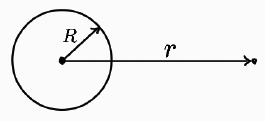
\includegraphics[width=0.45\textwidth]{monopole.png}
    \caption{Pulsating sphere (monopole) of radius \(R\). Sound radiation is omnidirectional and the radiated power depends on the ratio \(f/f_0\) where \(f_0 = c/(2\pi R)\)}
\end{figure}

\begin{figure}[!htb]
    \centering
    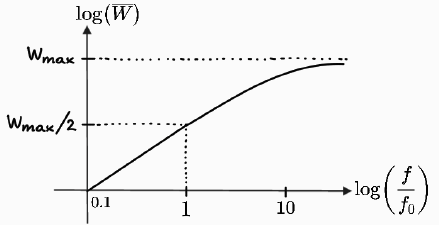
\includegraphics[width=0.50\textwidth]{log(W)(f).png}
    \caption{Mean radiated power \(\overline{W_A}\) of a pulsating sphere as a function of frequency on a logarithmic scale. Below the cutoff frequency \(f_0\), power falls as \(f^2\); above \(f_0\) it saturates at the plane-wave limit \(S\rho_0 c u_\mathrm{RMS}^2\)}
\end{figure}

The behavior of equation \eqref{eq:spherePower} has a clear physical interpretation. For \(f \gg f_0\) (i.e., \(kR \gg 1\), the sphere is large compared to the wavelength): \(\overline{W_A} \approx S \rho_0 c u_\mathrm{RMS}^2\), which is exactly the plane-wave result. The radiation is efficient and the specific impedance approaches the purely resistive value \(\rho_0 c\). For \(f \ll f_0\) (i.e., \(kR \ll 1\), the sphere is small compared to the wavelength): \(\overline{W_A} \propto (f/f_0)^2 \propto f^2\), so the radiated power falls off quadratically with decreasing frequency. In this regime the source is acoustically compact: the surrounding air is moved back and forth but the pressure perturbation cancels almost completely over the sphere's surface, and little net energy is radiated.

\paragraph{Physical meaning of the cutoff frequency} The frequency \(f_0 = c/(2\pi R)\) marks the transition between the mass-controlled regime (\(f \ll f_0\), reactive loading dominates) and the resistance-controlled regime (\(f \gg f_0\), efficient radiation). A critical consequence is that a source oscillating at zero frequency (\(f = 0\)) radiates zero acoustic power: steady motion of the surface merely displaces air without creating any propagating wave. Sound requires temporal variation of the source velocity; the faster the oscillation relative to \(f_0\), the more efficiently the source couples to the medium.
For a typical woofer with diaphragm radius \(a = \SI{10}{\centi\meter}\), the equivalent monopole cutoff frequency is \(f_0 = c/(2\pi a) \approx \SI{550}{\hertz}\). Below this frequency, the radiation resistance falls as \(f^2\) and the reactive (mass) part of the radiation impedance increasingly dominates the load seen by the diaphragm.

\section{Rigid Circular Piston in Infinite Baffle}
\label{sc:62}

A more accurate model for a real loudspeaker cone is the rigid circular piston of radius \(a\) mounted flush in an infinite, rigid, perfectly reflecting baffle. The baffle prevents rear-wave cancellation and constrains radiation to a half-space (\(2\pi\) steradians). This is also the reference geometry for which the radiation impedance is tabulated and against which real loudspeakers are often compared.

\begin{figure}[!htb]
    \centering
    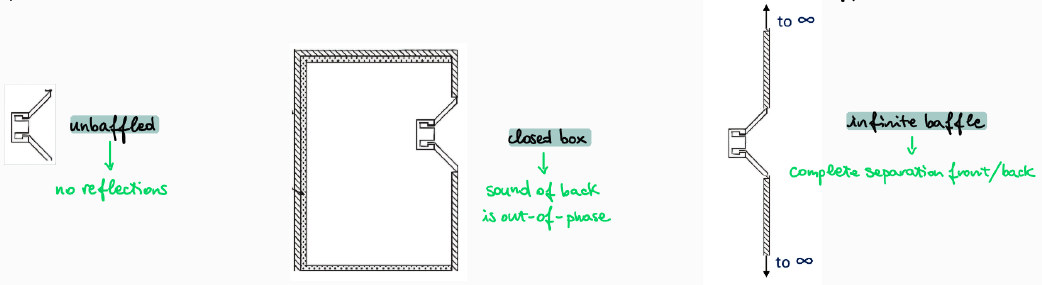
\includegraphics[width=0.65\textwidth]{rigid_piston_model.png}
    \caption{Rigid circular piston of radius \(a\) in an infinite baffle. The baffle prevents front-to-back acoustic short-circuiting, so radiation is restricted to the forward half-space. Different baffle configurations (infinite, finite, closed box) produce different radiation impedances and directivity patterns}
\end{figure}

\subsection{Far-Field Pressure and Directivity Function}
\label{ssc:621}

In the far field (\(r \gg a\)), the acoustic pressure radiated by the piston at a point \((r, \theta)\) in spherical coordinates is:
\[
\tilde{p}(r,\theta) = -j k a^2 \rho_0 c \tilde{u}_0 \frac{e^{-jkr}}{2r}\;D(\theta)
\]
where \(\tilde{u}_0\) is the complex piston velocity amplitude and \(D(\theta)\) is the directivity function:
\begin{equation}
    D(\theta) = \frac{2 J_1(ka\sin\theta)}{ka\sin\theta}
    \label{eq:directivity}
\end{equation}
Here \(J_1(\cdot)\) is the Bessel function of the first kind of order 1. On the axis (\(\theta = 0\)), \(D(0) = 1\) by the limit \(\lim_{x\to 0} 2J_1(x)/x = 1\), so the on-axis pressure is maximum and the expression simplifies to:
\[
\tilde{p}(r,0) = -j \rho_0 f \tilde{U}_0 \frac{e^{-jkr}}{2}, \qquad \tilde{U}_0 = \pi a^2 \tilde{u}_0
\]
where \(\tilde{U}_0\) is the volume velocity.

\subsection{The Parameter ka and Frequency-Dependent Behavior}
\label{ssc:622}

The dimensionless parameter \(ka\) controls all aspects of the piston's radiation:
\begin{equation}
    ka = \frac{2\pi a}{\lambda} = \frac{2\pi f a}{c} = \frac{f}{f_0}, \qquad f_0 = \frac{c}{2\pi a}
    \label{eq:ka}
\end{equation}
It expresses the ratio of the piston circumference \(2\pi a\) to the acoustic wavelength \(\lambda\), or equivalently the ratio of the operating frequency \(f\) to the characteristic frequency \(f_0\). The following table gives representative values of \(f_0\) for typical loudspeaker sizes:

\begin{table}[!htb]
\centering
\renewcommand{\arraystretch}{1.3}
\begin{tabular}{cc}
\hline
\textbf{Piston radius \(a\) (cm)} & \textbf{Cutoff frequency \(f_0\) (Hz)} \\
\hline
1  & 5500 \\
10 & 550  \\
30 & 183  \\
\hline
\end{tabular}
\caption{Characteristic cutoff frequency \(f_0 = c/(2\pi a)\) for three piston radii at \(c = \SI{343}{\meter\per\second}\)}
\end{table}

\paragraph{Low-frequency regime (\(ka \ll 1\))} When the piston diameter is much smaller than the wavelength, the Bessel function argument \(ka\sin\theta \ll 1\) for all angles, and \(D(\theta) \approx 1\) uniformly across the hemisphere: the radiation pattern is nearly omnidirectional. The source behaves as an acoustic monopole, and the radiated power falls as \(f^2\), exactly as for the pulsating sphere. The acoustic loading on the piston is predominantly reactive (mass-like), so the diaphragm is moving mostly against the inertia of the air rather than doing useful radiating work.

\begin{figure}[!htb]
    \centering
    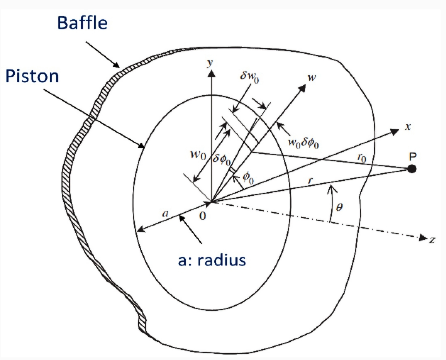
\includegraphics[width=0.45\textwidth]{rigid_piston.png}
    \caption{Rigid circular piston of radius \(a\) in an infinite baffle, showing the geometry for the far-field directivity calculation. The observation point P is at distance \(r\) and angle \(\theta\) from the piston axis}
\end{figure}

\paragraph{High-frequency regime (\(ka \gg 1\))} When the piston diameter is much larger than the wavelength, the zeros of \(J_1(ka\sin\theta)\) occur at angles progressively closer to the axis, and the radiation pattern narrows into a sharply focused main lobe along \(\theta = 0\) with increasingly numerous sidelobes at larger angles. In this regime the radiation resistance approaches the plane-wave value \(\rho_0 c\) and radiation is efficient, but it is concentrated in a narrow beam. From a practical standpoint, a large woofer operating at high frequencies radiates almost exclusively on-axis, causing severe high-frequency dispersion problems in the listening room.

\begin{figure}[!htb]
    \centering
    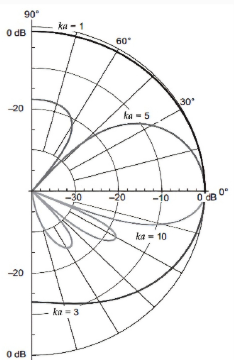
\includegraphics[width=0.40\textwidth]{directivity.png}
    \caption{Polar directivity pattern of a rigid circular piston for several values of \(ka\). For \(ka \ll 1\) the pattern is omnidirectional; as \(ka\) increases the radiation narrows into a progressively sharper main lobe with sidelobes}
\end{figure}

\subsection{Radiation Impedance of the Piston}
\label{ssc:623}

The specific radiation impedance seen by the piston surface is:
\begin{equation}
    Z_s = \frac{\tilde{F}}{\tilde{U}_0} = R_s + jX_s
    \label{eq:pistonImpedance}
\end{equation}
where the exact expressions in terms of Bessel and Struve functions are:
\[
R_s = \rho_0 c\left(1 - \frac{J_1(2ka)}{ka}\right), \qquad X_s = \rho_0 c \frac{\mathbf{H}_1(2ka)}{ka}
\]
with \(J_1(\cdot)\) the Bessel function of the first kind and \(\mathbf{H}_1(\cdot)\) the Struve function of the first kind. The mean acoustic power radiated by the piston is:
\[
\overline{W_A} = R_s S_D u_{0,\mathrm{RMS}}^2, \qquad S_D = \pi a^2
\]
For \(ka \ll 1\), the low-frequency asymptotic behavior of the radiation impedance components is:
\[
R_s \approx \frac{\rho_0}{2c} a^2 \omega^2 \propto \omega^2, \qquad X_s \approx \frac{8}{3\pi} a \rho_0 \omega \propto \omega
\]
The radiation resistance rises as \(\omega^2\) at low frequencies, confirming the \(f^2\) dependence of the radiated power for a velocity-driven piston. The radiation reactance rises as \(\omega\), behaving like the reactance of a mass \(M_{A1} = 8\rho_0 a/(3\pi^2)\) per unit area.

\begin{figure}[!htb]
    \centering
    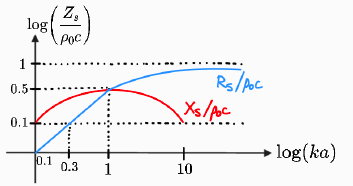
\includegraphics[width=0.75\textwidth]{acoustic_impedance_graph.png}
    \caption{Normalized specific radiation impedance \(Z_s/(\rho_0 c)\) for a rigid circular piston in an infinite baffle, plotted versus \(ka\) on a logarithmic scale. The resistive part \(R_s/(\rho_0 c)\) rises as \(\omega^2\) for \(ka \ll 1\) and saturates near unity for \(ka \gg 1\); the reactive part \(X_s/(\rho_0 c)\) rises as \(\omega\) for small \(ka\) and oscillates for large \(ka\)}
\end{figure}

\section{Acoustic End Correction: The Air Mass Load}
\label{sc:63}

The analysis of the piston's radiation impedance reveals that the reactive part \(X_s\), which rises linearly with frequency at low \(ka\), is equivalent to the reactance of an additional mass of air that must be accelerated every time the diaphragm moves. This air mass is not negligible: it represents a real physical contribution to the moving system of the loudspeaker that is not accounted for in the bare mechanical model of Chapter 4.

\subsection{The Acoustic End Correction Mass}
\label{ssc:631}

For a baffled piston at low frequencies (\(ka \ll 1\)), the reactive part of the radiation impedance per unit area is \(X_s = (8/3\pi) \rho_0 a \omega\). This is identical to the reactance of an acoustic mass:
\begin{equation}
    M_{A1} = \frac{8}{3\pi^2} \frac{\rho_0}{a} \quad \left[\si{\kilo\gram\per\meter\tothe{4}}\right]
    \label{eq:acousticMassA1}
\end{equation}
Referring this acoustic mass back to the mechanical domain through the diaphragm area \(S_D = \pi a^2\):
\begin{equation}
    M_{M1} = M_{A1} S_D^2 = \frac{8}{3\pi^2} \frac{\rho_0}{a}\cdot(\pi a^2)^2 = \frac{8\pi}{3} \rho_0 a^3 \approx 2.67 \rho_0 a^3 \quad [\si{\kilo\gram}]
    \label{eq:mechanicalEndCorrection}
\end{equation}
This result has a transparent geometric interpretation: \(M_{M1} = \rho_0\cdot\pi a^2\cdot(8a/3\pi) = \rho_0\cdot S_D\cdot(0.85 a)\), which is the mass of a column of air of cross-section \(S_D\) and effective length \(0.85 a\). The diaphragm does not move in isolation: it drags with it a cylinder of air whose length is approximately 85\% of the piston radius. This is the acoustic end correction, classically derived from potential flow theory.

\begin{figure}[!htb]
    \centering
    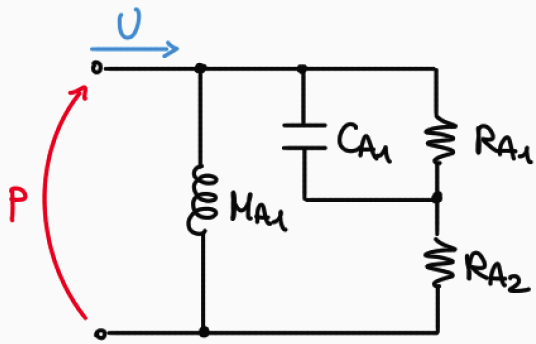
\includegraphics[width=0.65\textwidth]{radiation_circuit.png}
    \caption{Equivalent circuit at low frequencies showing the air mass \(M_{M1}\) in series with the radiation resistance \(R_{MR}\). The factor of 2 in the full expression \(2M_{M1}\) accounts for the air on both the front and rear faces of the loudspeaker when no baffle or enclosure is present}
\end{figure}

\subsection{Effect on the Total Moving Mass and Resonance Frequency}
\label{ssc:632}

The total moving mass of the loudspeaker system \(M_{MS}\) includes the diaphragm mass \(M_{MD}\) plus the air mass contributions from the front and rear radiation environments. For a loudspeaker mounted in an infinite baffle (open back), the front face carries an end correction \(M_{M1}\) and the rear face (which radiates into the enclosed air or free space behind the baffle) carries a second mass \(M_{M1}\), so:
\[
M_{MS} = M_{MD} + 2 M_{M1}
\]
For a driver in free air (no baffle at all), the same factor of 2 applies. In a closed-box enclosure, the rear air mass is modified by the acoustic compliance of the enclosure volume.
Since the air mass \(M_{M1} = 2.67 \rho_0 a^3\) scales with the cube of the piston radius, it becomes increasingly significant for larger drivers. For a \SI{10}{\centi\meter} radius woofer:
\[
M_{M1} = 2.67 \times \SI{1.2}{\kilo\gram\per\cubic\meter} \times (\SI{0.1}{\meter})^3 \approx \SI{3.2}{\gram}
\]
This value is comparable to the diaphragm mass of a typical woofer (5 to 15 grams), so the air mass correction is not a minor perturbation but a substantial fraction of the total moving mass.
The consequence for the system resonance frequency is direct. From Chapter 4, the free-air resonance frequency in the absence of any radiation load is:
\[
f_{s,\mathrm{bare}} = \frac{1}{2\pi\sqrt{M_{MD} C_{MS}}}
\]
When the air mass is included, the effective moving mass increases and the resonance frequency drops:
\begin{equation}
    f_s = \frac{1}{2\pi\sqrt{M_{MS} C_{MS}}} = \frac{1}{2\pi\sqrt{(M_{MD} + 2M_{M1}) C_{MS}}} < f_{s,\mathrm{bare}}
    \label{eq:resonanceWithAirMass}
\end{equation}
The parameter \(f_s\) measured on a physical loudspeaker (for instance from the impedance peak) already includes the air mass contribution, so it directly yields \(M_{MS}\) rather than the bare diaphragm mass \(M_{MD}\). When Thiele-Small parameters are extracted from impedance measurements, the quoted \(M_{MS}\) is the total moving mass including the air load.

\begin{figure}[!htb]
    \centering
    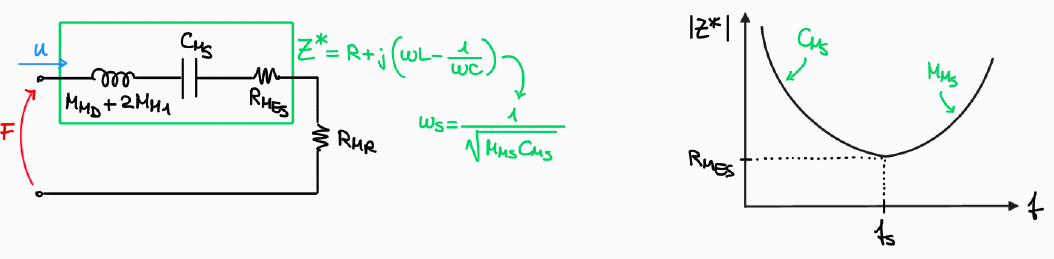
\includegraphics[width=0.80\textwidth]{low_freq_equiv.png}
    \caption{Low-frequency equivalent circuit of the loudspeaker including the air mass \(M_{M1}\). The total moving mass \(M_{MS} = M_{MD} + 2M_{M1}\) determines the resonance frequency \(f_s\) of the complete system. The radiation resistance \(R_{MR} \propto \omega^2\) rises steeply at low frequencies and falls far below the suspension damping \(R_{MS}\) at the resonance frequency of most practical woofers}
\end{figure}

\paragraph{Physical picture} The air in front of the cone is not acoustically transparent. When the diaphragm moves forward, it must accelerate a plug of air of finite mass before that mass can propagate its displacement outward as a sound wave. At low frequencies this plug moves back and forth with the cone but radiates very little power (because \(R_s \propto \omega^2\) is small), behaving as a purely inertial load. At frequencies above \(f_0 = c/(2\pi a)\), the air plug can no longer keep up with the cone and begins to decouple: the radiation resistance rises toward \(\rho_0 c\) and efficient sound radiation begins. The loudspeaker designer must therefore choose the diaphragm radius and resonance frequency such that the operating bandwidth falls in the transition region where radiation is efficient but directivity is not yet excessive.
